\documentclass[border=2mm]{standalone}
\usepackage{tikz}
\usetikzlibrary{calc,patterns,angles,quotes}
\begin{document}
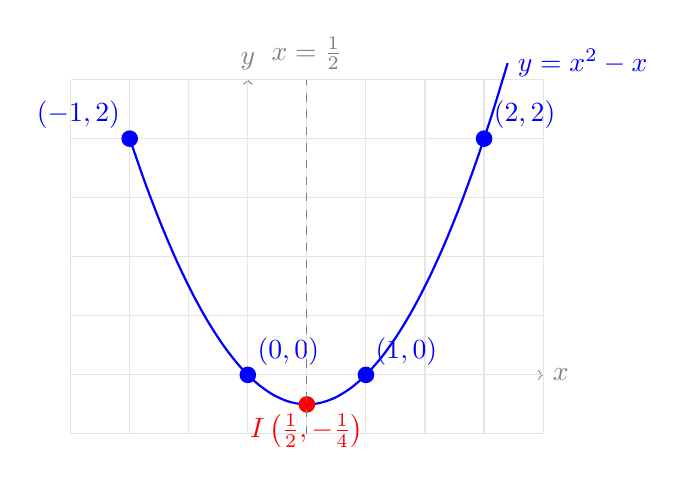
\begin{tikzpicture}[scale=1.5]
% Tọa độ các điểm quan trọng
\coordinate (O) at (0,0);
\coordinate (A) at (1,0);
\coordinate (I) at (0.5,-0.25);
\coordinate (B) at (2,2);
\coordinate (C) at (-1,2);

% Trục tọa độ
\draw[->, gray] (-1.5,0) -- (2.5,0) node[right] {$x$};
\draw[->, gray] (0,-0.5) -- (0,2.5) node[above] {$y$};

% Lưới mờ (tùy chọn)
\draw[gray!20, step=0.5] (-1.5,-0.5) grid (2.5,2.5);

% Vẽ parabol
\draw[blue, thick, domain=-1:2.2, smooth, variable=\x] plot ({\x}, {\x*\x - \x}) node[right] {$y=x^2-x$};

% Đánh dấu các điểm
\fill[blue] (O) circle (2pt) node[above right] {$(0,0)$};
\fill[blue] (A) circle (2pt) node[above right] {$(1,0)$};
\fill[red] (I) circle (2pt) node[below] {$I\left(\frac{1}{2},-\frac{1}{4}\right)$};

% Trục đối xứng (nét đứt)
\draw[gray, dashed] (0.5,-0.5) -- (0.5,2.5) node[above] {$x=\frac{1}{2}$};

% Ghi chú thêm một số điểm phụ
\fill[blue] (B) circle (2pt) node[above right] {$(2,2)$};
\fill[blue] (C) circle (2pt) node[above left] {$(-1,2)$};
\end{tikzpicture}
\end{document}